% Author: Giulio Stramondo, Mail: giuliostramondo[at]gmail.com
\documentclass{standalone}
\usepackage{tikz}
\usetikzlibrary{shapes.gates.logic.US,shapes.geometric,trees,positioning,arrows,calc}
\begin{document}
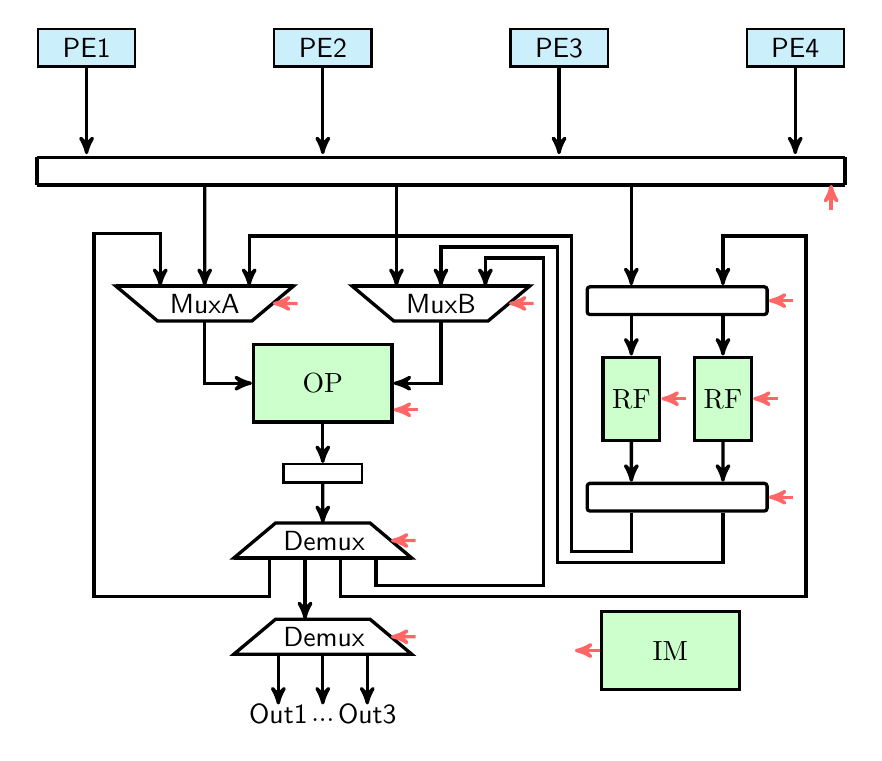
\begin{tikzpicture}[
% Gates and symbols style
    and/.style={and gate US,thick,draw,fill=red!60,rotate=90,
		anchor=east,xshift=-1mm},
    or/.style={or gate US,thick,draw,fill=blue!60,rotate=90,
		anchor=east,xshift=-1mm},
    archr/.style={rectangle,thick,draw,fill=red!60,anchor=north,
		minimum width=0.2cm},
    archb/.style={rectangle,thick,draw,fill=blue!60,anchor=north,
		minimum width=0.2cm},
    archm/.style={rectangle,thick,draw,fill=magenta!60,anchor=north,
		minimum width=0.2cm},
    select/.style={circle,thick,draw,anchor=north,
		minimum width=0.4cm},
    tr/.style={buffer gate US,thick,draw,fill=purple!60,rotate=90,
		anchor=east,minimum width=0.8cm},
    multiplexer/.style={
        draw,
        trapezium,
        %shape border uses incircle, 
        shape border rotate=180,
        %minimum size=18pt,
        %minimum height = 0.25cm,
        inner sep=1mm,
        outer sep=0mm,
        text width=1cm,
        align=center,
        font=\sffamily,
        minimum width = 0.5cm,
        trapezium left angle=40,
        trapezium right angle=40
    }, 
    demultiplexer/.style={
        draw,
        trapezium,
        %shape border uses incircle, 
        shape border rotate=0,
        %minimum size=18pt,
        %minimum height = 0.25cm,
        inner sep=1mm,
        outer sep=0mm,
        text width=1cm,
        align=center,
        font=\sffamily,
        minimum width = 0.5cm,
        trapezium left angle=40,
        trapezium right angle=40          
    },
% Label style
    label distance=3mm,
    every label/.style={blue},
% Event style
    event/.style={rectangle,thick,draw,fill=cyan!20,text width=1cm,
		text centered,font=\sffamily,anchor=north},
% Children and edges style
    edge from parent/.style={very thick,draw=black!70},
    edge from parent path={(\tikzparentnode.south) -- ++(0,-1.05cm)
			-| (\tikzchildnode.north)},
    level 1/.style={sibling distance=7cm,level distance=1.4cm,
			growth parent anchor=south,nodes=event},
    level 2/.style={sibling distance=7cm},
    level 3/.style={sibling distance=6cm},
    level 4/.style={sibling distance=3cm}
%  For compatability with PGF CVS add the absolute option:
   absolute
    ]
%% Draw events and edges
%    \node (g1) [event] {No flow to receiver}
%	     child{node (g2) {No flow from Component B}
%	     	child {node (g3) {No flow into Component B}
%	     	   child {node (g4) {No flow from Component A1}
%	     	      child {node (t1) {No flow from source1}}
%	     	      child {node (b2) {Component A1 blocks flow}}
%			}
%	     	   child {node (g5) {No flow from Component A2}
%	     	      child {node (t2) {No flow from source2}}
%	     	      child {node (b3) {Component A2 blocks flow}}
%			}
%		   }
%	     	child {node (b1) {Component B blocks flow}}
%		};
%%% Place gates and other symbols
%%% In the CVS version of PGF labels are placed differently than in PGF 2.0
%%% To render them correctly replace '-20' with 'right' and add the 'absolute'
%%% option to the tikzpicture environment. The absolute option makes the
%%% node labels ignore the rotation of the parent node.
%   \node [or]	at (g2.south)	[label=-20:G02]	{};
%   \node [and]	at (g3.south)	[label=-20:G03]	{};
%   \node [or]	at (g4.south)	[label=-20:G04]	{};
%   \node [or]	at (g5.south)	[label=-20:G05]	{};
%   \node [be]	at (b1.south)	[label=below:B01]	{};
%   \node [be]	at (b2.south)	[label=below:B02]	{};
%   \node [be]	at (b3.south)	[label=below:B03]	{};
%   \node [tr]	at (t1.south)	[label=below:T01]	{};
%   \node [tr]	at (t2.south)	[label=below:T02]	{};
%%% Draw system flow diagram
   \begin{scope}[xshift=-7.5cm,yshift=-5cm,very thick,
		node distance=3cm,on grid,>=stealth',
		block/.style={rectangle,draw,fill=green!20, minimum height=28pt, minimum width=50pt},
		comp/.style={circle,draw,fill=orange!40}]
       \node [event] (mul4) 	at (0,0)	{PE1};
       \node [event] (mul5) 	[right=of mul4]	{PE2};
       \node [event] (mul6) 	[right=of mul5]	{PE3};
       \node [event] (mul7) 	[right=of mul6]	{PE4};

       %CROSSBAR
       \node [] (cbtl) [below=of mul4.south west, below=1cm]{};
       \node [] (cbtr) [below=of mul7.south east, below=1cm]{};
       \draw (cbtl.center) --  (cbtr.center); 
       \draw (cbtl.center) --  ++ (0,-10pt) coordinate (cbbl); 
       \draw (cbtr.center) --  ++ (0,-10pt) coordinate (cbbr); 
       \draw (cbbl.center) --  (cbbr.center); 
       %END CROSSBAR

       %LINKS
       \node [] (mul4hook) [below=of mul4.south, below=1.1cm]{};
       \node [] (mul5hook) [below=of mul5.south, below=1.1cm]{};
       \node [] (mul6hook) [below=of mul6.south, below=1.1cm]{};
       \node [] (mul7hook) [below=of mul7.south, below=1.1cm]{};
       \draw[->] (mul4.south) -- (mul4hook);
       \draw[->] (mul5.south) -- (mul5hook);
       \draw[->] (mul6.south) -- (mul6hook);
       \draw[->] (mul7.south) -- (mul7hook);
       \draw[-,opacity=0] (mul4hook.north) -- (mul5hook.north) node[pos=1/2] (mul45hook){};

       \node [] (mul45hooklow) [below=of mul45hook,below=0.1cm]{};
       \node [] (mul56hooklow) [right=of mul45hooklow]{};
       \node [multiplexer] at ([yshift=-50pt]mul45hook.south) (mux1) {MuxA};
       \draw [->] (mul45hooklow) -- (mux1.north);
       \node [multiplexer] [right=of mux1] (mux2) {MuxB};
       %\node [multiplexer] [right=of mux2] (mux3) {MuxRF};
       \node [rectangle, draw, minimum width=65pt, minimum height=10pt,rounded corners=1pt] [right=of mux2,yshift=1pt] (cbRF) {};
       %\node [demultiplexer] [below=of mux3,below=6mm] (dem3) {DemRF};
       %\draw[-] (dem3.bottom left corner) -- (dem3.bottom right corner)
       %         node [pos=2/8] (demrfhook1){}
       %         node [pos=6/8] (demrfhook2){};
       \draw[-,opacity=0] (cbRF.south west) -- (cbRF.south east)
                node [pos=2/8] (demrfhook1){}
                node [pos=6/8] (demrfhook2){};

       %\draw [->] (mux3) -- (dem3);
       \draw [-,opacity=0]
                (mux2.bottom left corner) -- (cbRF.north west)
                node [pos=1/4] (horizontaladdhook){}
                node [pos=2/4] (horizontalmuxbhook){}
                node [pos=3/4] (horizontalmuxahook){};
       \draw [-,opacity=0] (cbRF.north west) -- (cbRF.north east)
            node [pos=2/8] (muxrfCrossbarHook){}
            node [pos=6/8] (muxrfAddDemux){};

       \draw let
            \p1 = (muxrfCrossbarHook),
            \p2 = (cbbr)
            in 
            node (crossbarMuxrfHook) at (\x1,\y2){};
        \draw[->] (crossbarMuxrfHook.center) -- (muxrfCrossbarHook.center);
       \node [block] (rf) [below=of demrfhook1,below=5mm,minimum width=20pt,minimum height=30pt] {RF};
       \node [block] (rf2) [below=of demrfhook2,below=5mm,minimum width=20pt,minimum height=30pt] {RF};
       \node [] (rfsmidpoint) at ($(rf)!0.5!(rf2)$) {};
       \node [rectangle, draw, minimum width=65pt, minimum height=10pt,rounded corners=1pt] [below=of rfsmidpoint,below=30pt] (cbRF2) {};
       \draw [-,opacity=0] (cbRF2.north west) -- (cbRF2.north east)
            node [pos=2/8] (cb2RFhook) {}
            node [pos=6/8] (cb2RF2hook) {};
        \draw[->] (rf) -- (cb2RFhook.center);
        \draw[->] (rf2) -- (cb2RF2hook.center);

        \draw[-,opacity=0] (cbRF2.south west) -- (cbRF2.south east)
            node [pos=2/8] (rfMuxA){}
            node [pos=6/8] (rfMuxB){};
       %\draw[-] (rf.south west) -- (rf.south east) node [pos=1/2] (rfMuxA){};
       %\draw[-] (rf2.south west) -- (rf2.south east) node [pos=1/2] (rfMuxB){};

       
       \node[] (rfMuxA1) [below=of rfMuxA,below=10pt] {};
       \node[] (rfMuxB1) [below=of rfMuxB,below=14pt] {};
       \draw let 
            \p1 = (horizontalmuxahook),
            \p2 = (rfMuxA1)
            in
        node (rfMuxA2) at (\x1,\y2) {};

        \draw let 
            \p1 = (horizontalmuxbhook),
            \p2 = (rfMuxB1)
            in 
        node (rfMuxB2) at (\x1,\y2){};
       \coordinate (coordrfMuxB2) at ($(rfMuxB1)+(rfMuxA2)-(rfMuxA1) +(rfMuxA)-(rfMuxB)+(rfMuxA)-(rfMuxB)$); 

       \node[] (rfMuxA3) [above=of rfMuxA2,above=110pt]{};

       \draw let 
            \p1 = (rfMuxA3),
            \p2 = (rfMuxB2),
            \p3 = (rfMuxA2)
            in
        node (rfMuxB3) at ($(\x2,\y1)- (0,\y3)+(0,\y2)$){};
        \draw [->] (demrfhook1.center)->(rf);
        \draw [->] (demrfhook2.center)->(rf2);
       
       \draw [-] (mux2.bottom right corner) -- (mux2.bottom left corner) node [pos=1/4](mux2crossbarhook){};
       \draw [-] (mux2.bottom right corner) -- (mux2.bottom left corner) node [pos=2/4](mux2RFhook){};
       \draw [-] (mux2.bottom right corner) -- (mux2.bottom left corner) node [pos=3/4](mux2Demuxhook){};
       \draw let 
            \p1 = (mux2RFhook),
            \p2 = (rfMuxB3)
            in
            node (rfMuxB4) at (\x1,\y2){};
       \draw[->] (rfMuxB.center) -- (rfMuxB1.center) -- (rfMuxB2.center) -- (rfMuxB3.center) -- (rfMuxB4.center) -- (mux2RFhook.center);
       \draw [-,fill=red] (mux1.bottom right corner) -- (mux1.bottom left corner)node[pos=3/4](muxahookrf){};
       \draw let 
            \p1 = (muxahookrf),
            \p2 = (rfMuxA3)
            in
            node (rfMuxA4) at (\x1,\y2){};
       \draw[->] (rfMuxA.center) -- (rfMuxA1.center) -- (rfMuxA2.center) -- (rfMuxA3.center) -- (rfMuxA4.center) -- (muxahookrf.center);

       \draw let 
            \p1 = (muxrfAddDemux),
            \p2 = (rfMuxA3)
            in 
            node (muxrfAddDemux2) at ( \x1,\y2){}
            node (muxrfAddDemux3) at ($(\x1,\y2) + (30pt,0) $){};
       \draw let
            \p1 = (mul56hooklow.south),
            \p2 = (mux2crossbarhook)
            in
       node (crossbarMux2hook) at (\x2,\y1){};

       \draw [->] (crossbarMux2hook.center) -- (mux2crossbarhook.center);
       \draw [-,opacity=0] (mux1) -- (mux2) node[pos=1/2](mux12mid){};
       \node [block] (op) [below=of mux12mid,below=5mm] {OP};
       \draw [->] (mux1) |- (op.west);
       \draw [->] (mux2) |- (op.east);
       \node [rectangle,thick,draw,minimum width=1cm] (ff) [below=of op.south,below=5mm] {};
       \draw [->] (op) -- (ff);
       \node [demultiplexer, minimum height=0.3cm](demuxadd) [below=of ff.south,below=5mm]{Demux};
       \draw [->] (ff) -- (demuxadd);
       \draw [-,fill=red] (demuxadd.bottom left corner) -- (demuxadd.bottom right corner)node[pos=1/5](muxahookdemux1){};
       \draw [-,fill=red] (demuxadd.bottom left corner) -- (demuxadd.bottom right corner)node[pos=2/5](muxahookdemux2){};
       \draw [-,fill=red] (demuxadd.bottom left corner) -- (demuxadd.bottom right corner)node[pos=3/5](muxahookdemux3){};
       \draw [-,fill=red] (demuxadd.bottom left corner) -- (demuxadd.bottom right corner)node[pos=4/5](muxahookdemux4){};

       \draw [-,fill=red] (mux1.bottom right corner) -- (mux1.bottom left corner)node[pos=1/4](muxahookdemux){};
        \node[] (demuxAdd1) [below=of muxahookdemux1.center,below=10pt]{}; 
        \node[] (demuxAdd4) [above=of muxahookdemux.center,above=15pt]{}; 
        \node[] (demuxAdd3) [left=of demuxAdd4.center,left=20pt]{}; 
        \draw let 
            \p1 = (demuxAdd1), 
            \p2 = (demuxAdd3) 
            in 
        node (demuxAdd2) at (\x2,\y1) {};
        \node[] (demuxAdd3) [left=of demuxAdd4.center,left=20pt]{};
        \draw [->] (muxahookdemux1.center) -- (demuxAdd1.center) -- (demuxAdd2.center) -- (demuxAdd3.center) -- (demuxAdd4.center) --(muxahookdemux.center);
        \node[demultiplexer] (demuxout) [below=of demuxadd,below=10mm]{Demux};
        \draw let
           \p1 = (muxahookdemux2),
           \p2 = (demuxout.north west)
           in
        node (demuxDemuxOut) at (\x1,\y2){};
        \draw[->] (muxahookdemux2.center) -- (demuxDemuxOut.center);
        \draw [-](demuxout.bottom left corner) -- (demuxout.bottom right corner) node [pos=1/4](demuxout1){};
        \draw [-](demuxout.bottom left corner) -- (demuxout.bottom right corner) node [pos=2/4](demuxout2){};
        \draw [-](demuxout.bottom left corner) -- (demuxout.bottom right corner) node [pos=3/4](demuxout3){};

        \draw let 
            \p1 = (demuxAdd1),
            \p2 = (muxahookdemux3),
            \p3 = (muxahookdemux4)
            in
            node (demuxAddRF1) at (\x2,\y1){}
            node (demuxAddMuxB) at ($(\x3,\y1) +(0,4pt)$){};

        \draw let 
            \p1 = (demuxAddRF1),
            \p2 = (muxrfAddDemux3)
            in
            node (muxrfAddDemux4) at (\x2,\y1){};

        \draw [->]
       (muxahookdemux3.center) -- (demuxAddRF1.center) -- (muxrfAddDemux4.center) -- (muxrfAddDemux3.center) -- (muxrfAddDemux2.center) -- (muxrfAddDemux.center);

        \draw let 
            \p1 = (horizontaladdhook),
            \p2 = (demuxAddMuxB)
            in
            node (demuxAddMuxB1) at (\x1,\y2){};
        \draw let
            \p1 = (demuxAddMuxB1),
            \p2 = (rfMuxB3),
            \p3 = (mux2Demuxhook)
            in
            node (demuxAddMuxB2) at ($(\x1,0)+(0,\y2)-(0,4pt) $){}
            node (demuxAddMuxB3) at ($(\x3,0)+(0,\y2)-(0,4pt) $){};
        \draw[->] (muxahookdemux4.center) -- (demuxAddMuxB.center) -- (demuxAddMuxB1.center) -- (demuxAddMuxB2.center) -- (demuxAddMuxB3.center) -- (mux2Demuxhook.center);

        
        \node[](demuxout1hook) [below=of demuxout1,below=5mm] {};
        \node[](demuxout1hookLabel) [below=of demuxout1hook.north,below=0pt,font=\sffamily] {Out1};
        \draw[->] (demuxout1.center) -- (demuxout1hook.center);

        \node[](demuxout2hook) [below=of demuxout2,below=5mm] {};
        \node[](demuxout2hookLabel) [below=of demuxout2hook.north,below=5pt] {...};
        \draw[->] (demuxout2.center) -- (demuxout2hook.center);

        \node[](demuxout3hook) [below=of demuxout3,below=5mm] {};
        \node[](demuxout3hookLabel) [below=of demuxout3hook.north,below=0pt,font=\sffamily] {Out3};
        \draw[->] (demuxout3.center) -- (demuxout3hook.center);

        \node [block] (im) [right=of demuxout,right=100pt,yshift=-5pt]{IM};
        \node [] (ctrl) [left=of im.west,left=5pt]{};
        \draw [->,draw=red!60] (im)-- (ctrl.center);

        \node [] (demuxoutctrl) [right=of demuxout.east,right=5pt]{};
        \draw [->,draw=red!60] (demuxoutctrl.center) -- (demuxout);

        \node [] (demuxaddctrl) [right=of demuxadd.east,right=5pt]{};
        \draw [->,draw=red!60] (demuxaddctrl.center) -- (demuxadd);

       %cbRF
        \node [] (cbRFctrl) [right=of cbRF.east,right=5pt]{};
        \draw [->,draw=red!60] (cbRFctrl.center) -- (cbRF);
        %cbRF2
        \node [] (cbRF2ctrl) [right=of cbRF2.east,right=5pt]{};
        \draw [->,draw=red!60] (cbRF2ctrl.center) -- (cbRF2);

        %rf
        \node [] (rfctrl) [right=of rf.east,right=5pt]{};
        \draw [->,draw=red!60] (rfctrl.center) -- (rf);

        %rf2
        \node [] (rf2ctrl) [right=of rf2.east,right=5pt]{};
        \draw [->,draw=red!60] (rf2ctrl.center) -- (rf2);

        %mux1
        \node [] (mux1ctrl) [right=of mux1.east,right=5pt]{};
        \draw [->,draw=red!60] (mux1ctrl.center) -- (mux1);

        %mux2
        \node [] (mux2ctrl) [right=of mux2.east,right=5pt]{};
        \draw [->,draw=red!60] (mux2ctrl.center) -- (mux2);

        %op
        \node [] (opctrl) [right=of op.south east,right=5pt,yshift=5pt]{};
        \coordinate (opctrlhook) at ($(op.south east) +(0,+5pt)$);
        \draw [->,draw=red!60] (opctrl.center) -- (opctrlhook);

        %cbbr
        \node [] (cbbrctrl) [below=of cbbr,below=5pt,xshift=-5pt]{};
        \coordinate (cbbrctrlhook) at ($(cbbr.center) +(-5pt,0)$);
        \draw [->,draw=red!60] (cbbrctrl.center) -- (cbbrctrlhook);

   \end{scope}
\end{tikzpicture}
\end{document}

